\documentclass[msc,proposal,hidelot,hideabstract]{ppgccufmg} % ou [msc] para dissertações
                                        % de mestrado. Para propostas ou
                                        % projetos, usar [phd,project],
                                        % [msc,proposal], etc.
\usepackage[brazil]{babel} % ajusta vários detalhes para
                           % documentos escritos em português,
                           % principalmente hifenização
\usepackage[T1]{fontenc}   % permite a hifenização de
                           % palavras acentuadas
\usepackage[utf8x]{inputenc} % ou [utf8x] para quem prefere
                             % usar a codificação UTF-8
\usepackage{graphicx} % define o comando \includegraphics
                      % para a inclusão de Figuras
%\usepackage[square]{natbib} % permite citações naturalmente
                            % integradas ao texto
\usepackage[a4paper,
portuguese,
bookmarks=true,
bookmarksnumbered=true,
linktocpage,
colorlinks=true,
citecolor=black,
urlcolor=black,
linkcolor=black,
filecolor=black,
]{hyperref}
\usepackage[table,xcdraw]{xcolor}

\begin{document}
\ppgccufmg{
title={Presto:\\
Diretrizes Construção de Sistemas para Extração de Relatórios de Negócio\\
no Contexto da XBRL},
author={Vagner Clementino},
university={Universidade Federal de Minas Gerais},
course={Ciência da Computação},
address={Belo Horizonte},
date={2015-05},
advisor={Rodolfo F. Resende},
abstract={Resumo}{resumo},
}
\chapter{Introdução}
\label{ch:Contexto}
No cenário atual, onde os sistemas de informação tem se tornado grandes e complexos, vemos a existência de um ecossistema de sistemas, também conhecidos como \textit{Systems of Systems} (SoS) \cite{Nakagawa:2013:SAF:2489850.2489853}. Organizações de grande porte, como os governos municipais, estaduais ou federal ou mesmo empresas multinacionais, precisam projetar sistemas de sistema ao invés vez de sistemas isolados a fim de enfrentar desafios tais como: $(i)$ colaboração entre organizações financiadas e geridas de forma independente; $(ii)$ migração para um ambiente orientado a serviços (SOA\footnote{Service Oriented Architecture }); $(iii)$ processos de testes e verificação da conformidade para sistemas de sistemas. Neste contexto, surge a necessidade do desenvolvimento de \textit{abordagens, técnicas e tecnologias} para a interação e evolução dos SoS.

No tocante a interoperabilidade de dados, diversos padrões vêm sendo propostos. Mais recentemente o formato JSON \cite{RFC4627} vêm crescendo em popularidade, contudo, o intercâmbio de dados é realizado primordialmente através da XML (Extensible Markup Language\footnote{\url{http://www.w3.org/XML/}}) e seus derivados. Na área medica, o padrão HL7 V3 message\footnote{\url{http://www.hl7.org/}} vêm sendo largamente adotado para troca de mensagem entre sistemas médicos \cite{Andrikopoulos:2013:TEO:2491845.2491890}{}. No contexto dos Sistemas de Informação Geográficas (SIG) a GML (Geography Markup Language\footnote{\url{http://www.opengeospatial.org/standards/gml}}) consolidou-se com o principal instrumento para interoperabilidade de dados geográficos \cite{gmlpaper}{}. Na área financeira diversas linguagens de marcação vêm sendo utilizadas para o intercâmbio de informações na Internet: \textit{Open Financial Exchange}\footnote{\url{http://www.ofx.net/}} (OFX), \textit{Eletronic Business Using XML}\footnote{\url{http://www.ebxml.org}} (ebXML), \textit{Financial Information eXchange}\footnote{\url{https://fixspec.com/}} (FIX), \textit{Market Data Definition Language}\footnote{\url{http://www.mddl.org}}, dentre outras \cite{xbrl_conceitos_aplicacoes}{}.

Com o advento da Web as linguagens de marcação cresceram em importância sobretudo devido a necessidade de se adicionar significado a informações sendo transferidas. Contudo, o padrão HTML (Hypertext
Markup Language) foi desenvolvido com objetivo de descrever \textit{como} a informação deve ser apresentada e não possui compromisso com o significado da informação. Nos meados da década de 1980,  a Organização para Padronização Internacional (ISO) propôs uma metalinguagem padrão a fim de etiquetar informações com conteúdo semântico. Esta linguagem foi denominada como \textit{Standard Generalized Markup Language} (SGML) \cite{smith1988sgml}.

A linguagem SGML, embora fosse capaz de definir diferentes tipos de marcação, a sua flexibilidade trouxe como preço a complexidade. O conceito era correto, todavia, havia a necessidade de ser mais simples. Com este objetivo em mente, um pequeno grupo de trabalho e um maior número de interessados começou a trabalhar em
meados dos anos 1990 em um subconjunto de SGML conhecido como \textit{Extensible Markup Language} (XML). A versão 1.0 foi publicada em 1996 e, dois anos mais tarde, o World Wide Web Consortium\footnote{\url{http://www.w3.org}} (W3C) publicou uma versão revisada \cite{Fawcett:2012:BX:2408362}{}.

Conforme exposto, a XML foi especificada a partir da SGML, na tentativa de se resolver as limitações da HTML
e da SGML. Neste sentido, um documento em XML pode ser publicado na Web, interpretado por pessoas
ou processado por aplicações. Apropriando-se desta características da XML, diversas linguagens vêm sendo propostas com a finalidade de troca de informações.

A XBRL (\textit{eXtensible Business Reporting Language}) é uma linguagem para divulgação e intercâmbio de informações financeiras baseada em XML\cite{xbrl_conceitos_aplicacoes}. O padrão vem sendo adotado por diversas instituições e empresas em todo mundo com o suporte de um consórcio global\footnote{\url{www.xbrl.org}} com mais de 650 membros que incentivam a criação de jurisdições locais. Atualmente o consórcio conta com 24 jurisdições, sendo que em países como  Estados Unidos, Grã-Bretanha e Austrália, a XBRL já é a linguagem oficial para entrega de relatórios à órgãos de governo. A Figura \ref{fig:world_map} exibe os países que estão promovendo a adoção da XBRL.

\begin{figure}[hbtp]
\centering
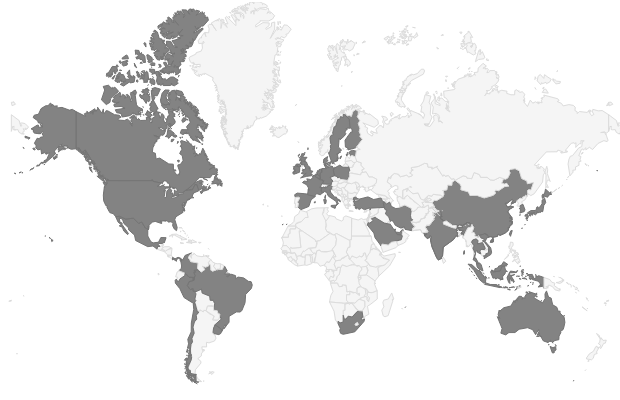
\includegraphics[width=.75\textwidth]{img/world-map.png}
\caption{O uso da XBRL no mundo}
\label{fig:world_map}
\end{figure}

Os estudos para definição da XBRL iniciaram em 1998 nos Estados Unidos pelo contador Charles Hoffman com apoio \textit{Institute of Certified Public Accountants} (AICPA). O objetivo era utilizar a XML para padronizar a divulgação de informações financeiras em formato eletrônico. A primeira versão do padrão, a XBRL 1.0, foi lançada em 2000, sendo a versão 2.0 lançada em dezembro de 2001. No mês de dezembro de 2003, foi lançada a versão 2.1 (\cite{hoffman_2006}), corrigindo algumas deficiências detectadas na versão anterior. A versão 2.1 se mantêm como a versão mais atual e estável da XBRL.

A linguagem XBRL define a estrutura básica dos documentos de instância, que são aqueles que portam os dados, e possibilita ainda a especificação de taxonomias que podem ser criadas para acomodar particularidades de cada organização por meio da introdução de novos elementos, denominados conceitos. Neste sentido, a linguagem possui elementos que facilitam a sua extensão e, por consequência, a adoção em diversos contextos.

Apesar de sua crescente adoção, falta à XBRL uma notação que facilite a sua modelagem e a comunicação entre as diferentes partes interessadas (\textit{`interessados"}. A necessidade de um modelo abstrato para a XBRL foi manifestada pelo próprio \textit{XBRL Consortium}. Em 2010 (\cite{xbrl_preserve_promote_particite}), o consórcio declarou que a criação de um modelo conceitual é uma das seis iniciativas que darão suporte a contínua adoção do padrão. Com o objetivo de preencher esta lacuna propõe neste documento o desenvolvimento de uma linguagem conceitual para a XBRL. A seguir descreve-se como o documento está estruturado.

No Capítulo \ref{ch:justificativa} discute-se as justificativas para adoção da XBRL bem como da criação de uma linguagem conceitual. O Capítulo \ref{ch:revisao} apresenta-se a revisão da literatura no tocante a criação de ontologias em diversos campos dos conhecimento, especialmente para área financeira e contábil. No Capítulo \ref{ch:metodologia} é discutida a metologia a ser aplicada. No Apêndice \ref{attch:cronograma} é exibido o cronograma do trabalho.

\chapter{Justificativa}
\label{ch:justificativa}

Nas organizações as informações contábeis e financeiras são armazenadas em diversos formatos (planilhas eletrônicas, documentos de texto, bancos de dados relacionais e etc). Não obstante, se faz necessário a transformação destas informações em um formato único a fim de facilitar a sua recuperação bem como a sua transmissão para outros sistemas. O processo de transformação e redirecionamento da informação internamente na organização, entre a organização e sua filiais ou mesmo entre a empresa e os governos. Este fluxo de informação, especialmente para a geração de relatórios, é exibido na Figura \ref{fig:fluxo_dados}.

\begin{figure}[hbtp]
\centering
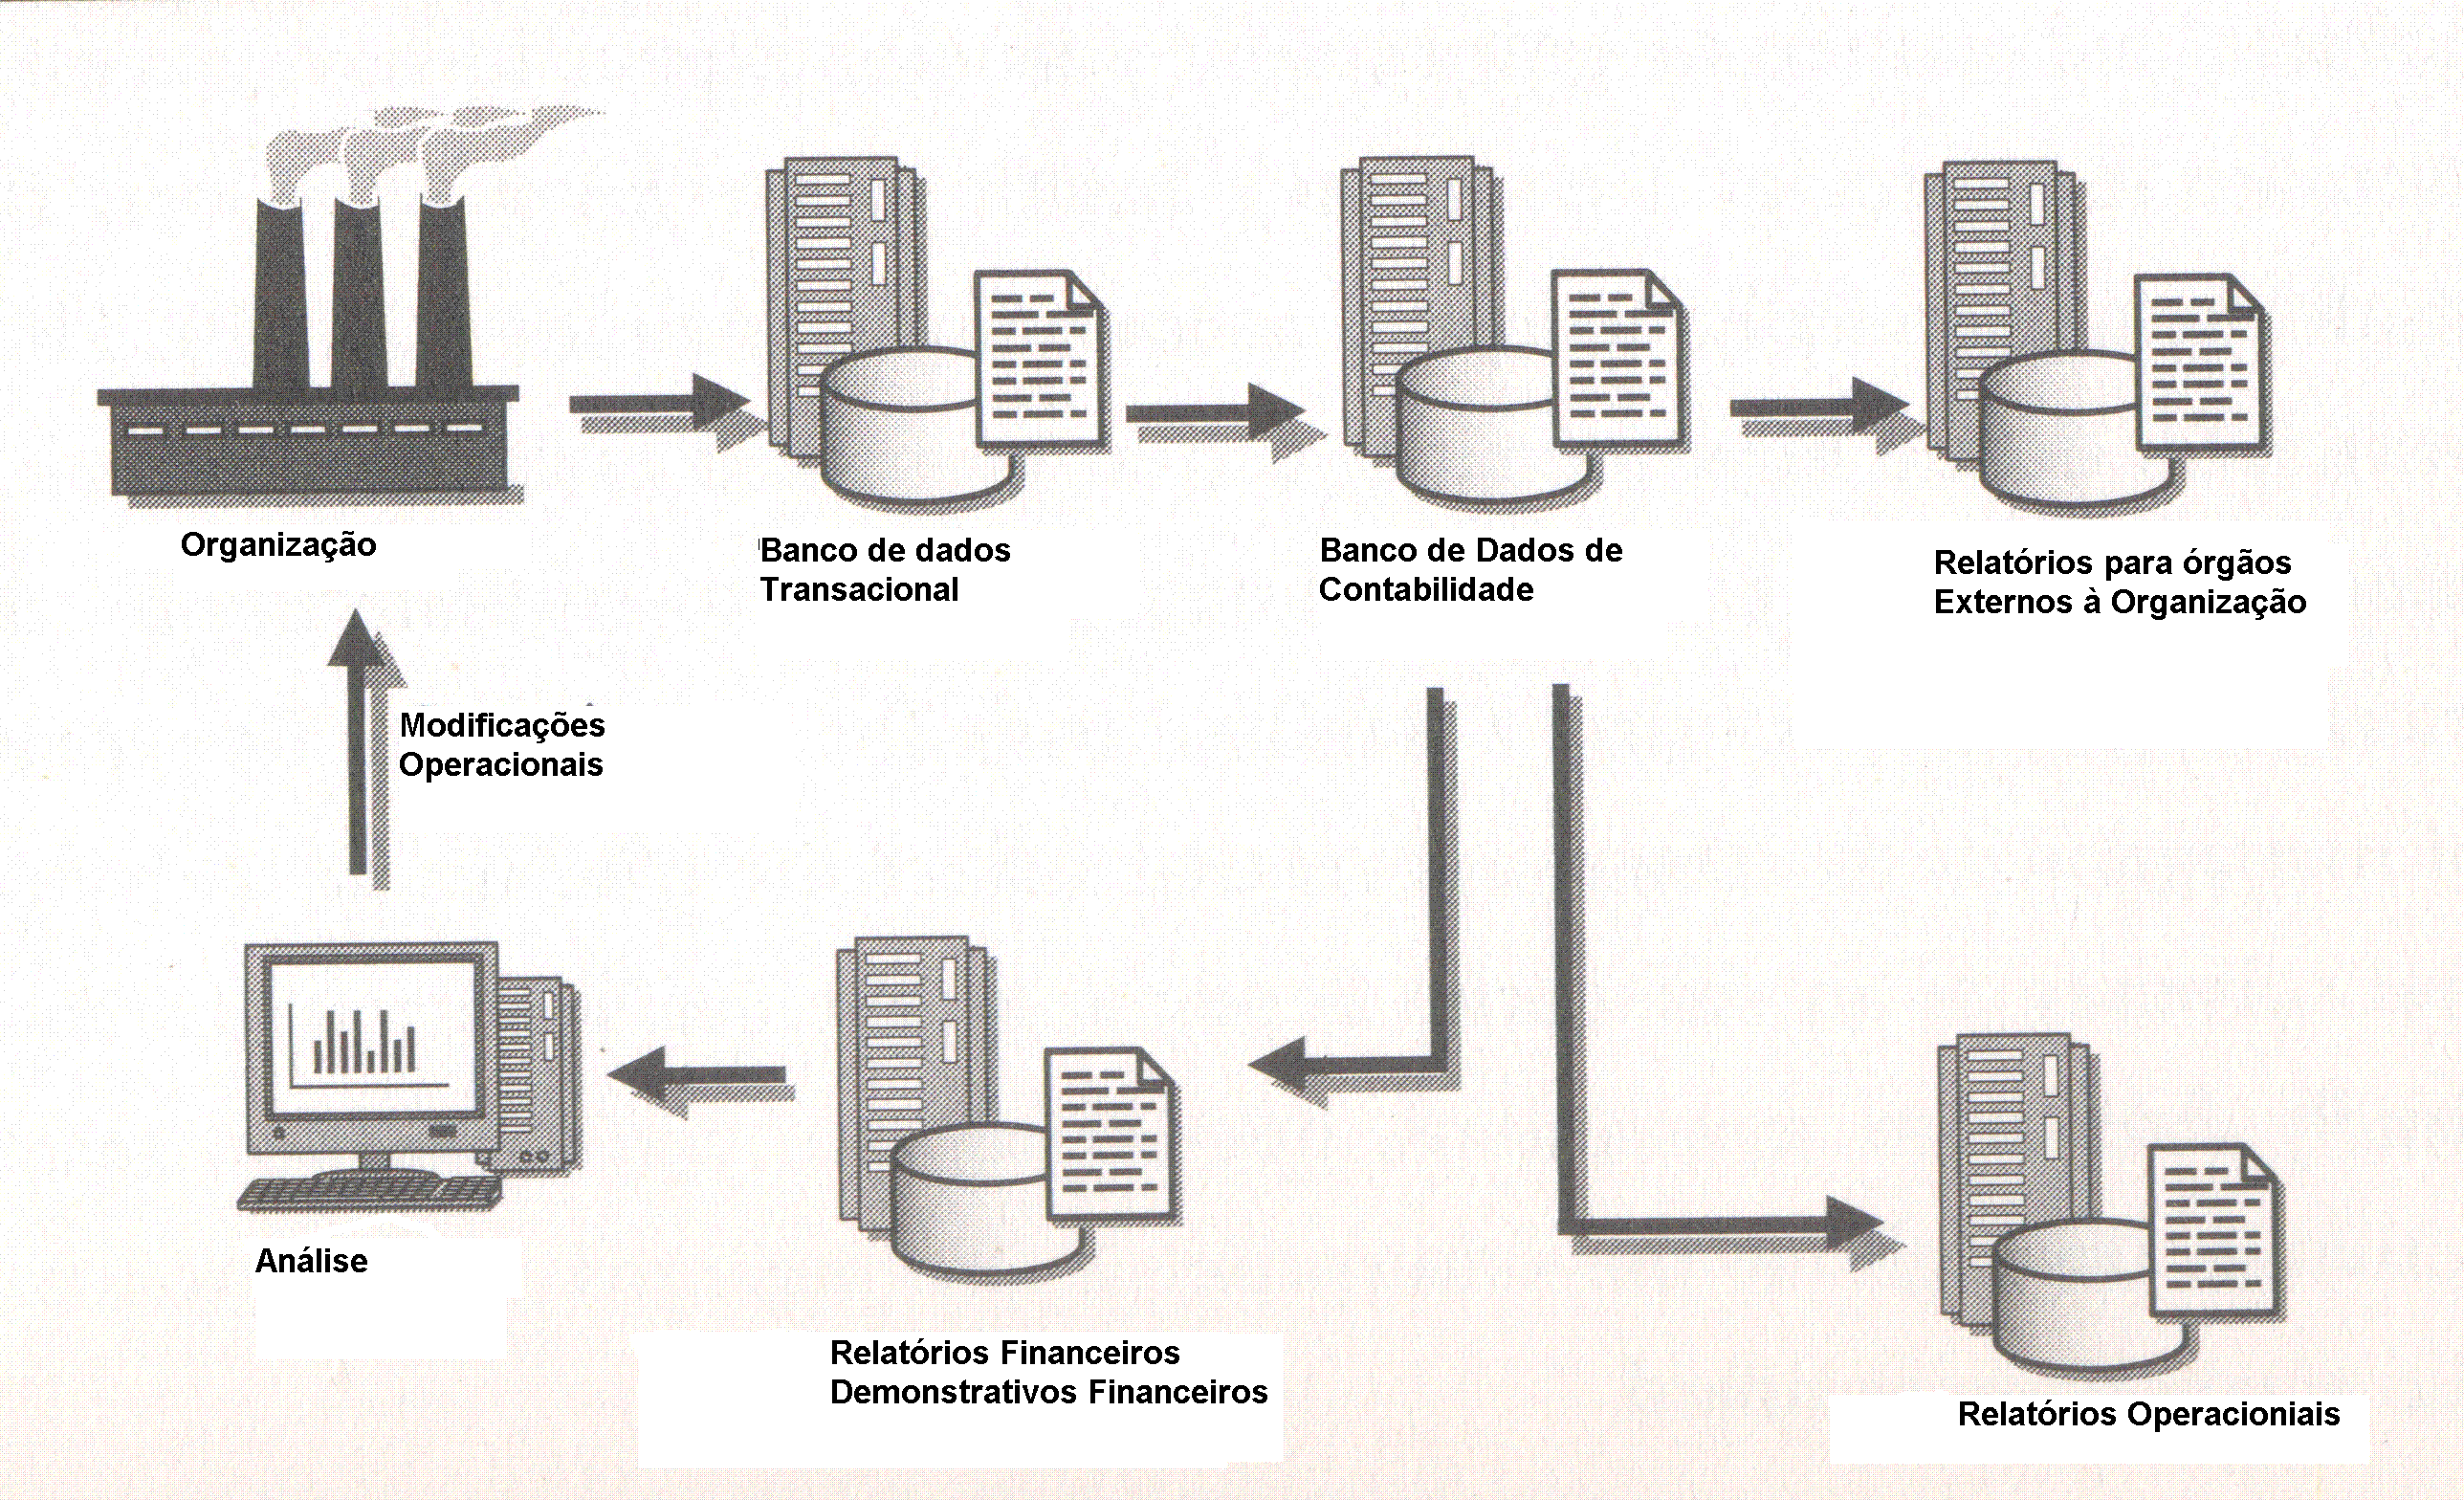
\includegraphics[width=.75\textwidth]{img/fluxo_informacoes.png}
\caption{Fluxo de dados financeiros em uma organização. Adaptado de (\cite{bergeron2004essentials}).}
\label{fig:fluxo_dados}
\end{figure}

Se pensarmos em uma organização que necessita receber informações de diversos locais, como por exemplo o governo federal de um país que solicite a prestação de contas de estados e municípios, onde cada ente possui seu próprio sistema para registro dos fatos financeiros. Neste contexto, haverá a necessidade de se criar diferentes interfaces para a conversão de formatos e padrões de contabilização. A Figura \ref{fig:interfaces} ilustra este cenário.


\begin{figure}[hbtp]
\centering
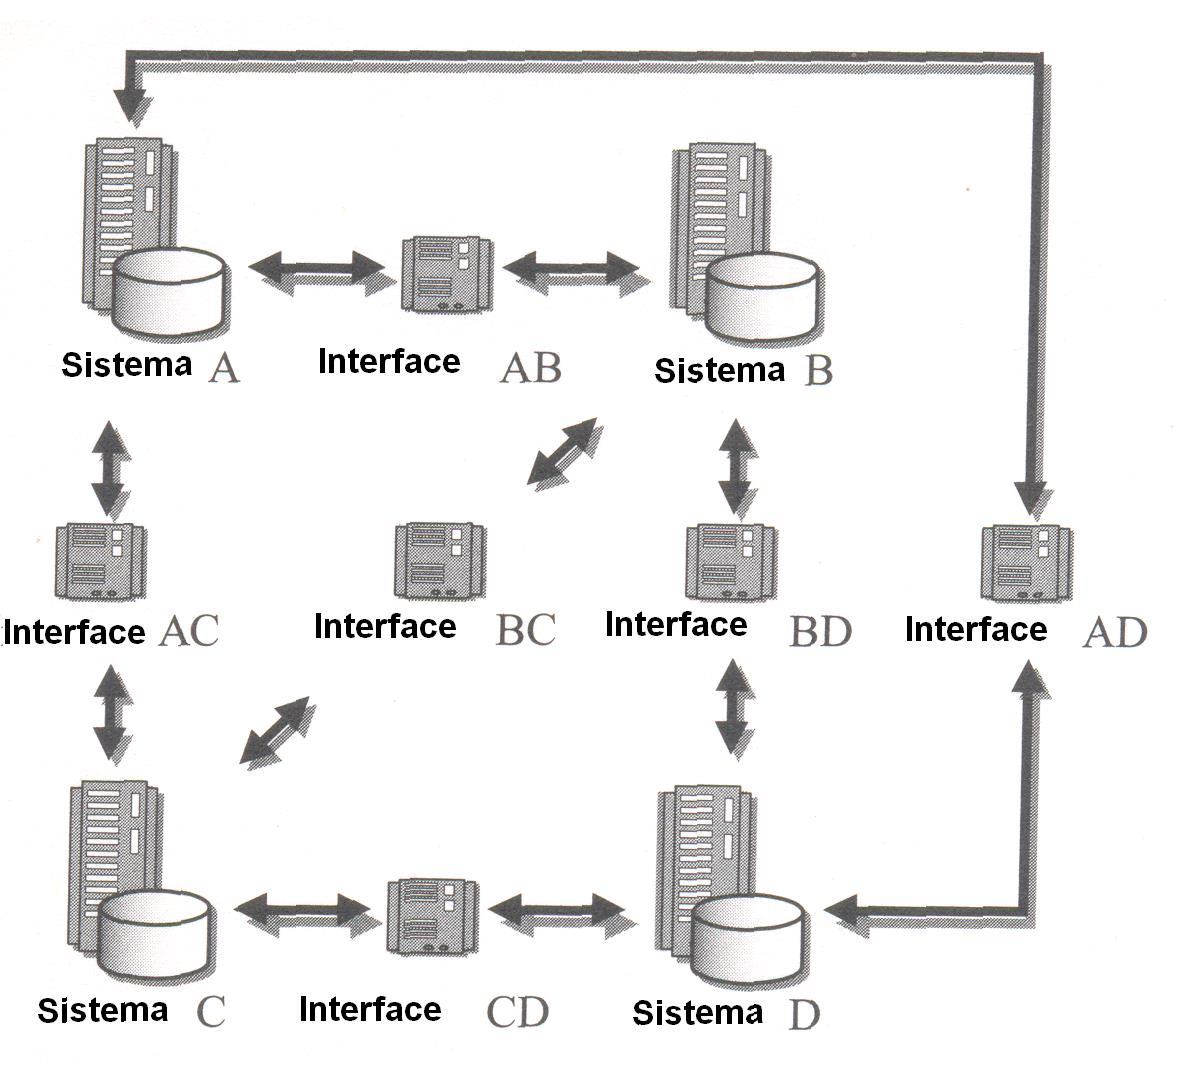
\includegraphics[width=.75\textwidth]{img/interfaces.png}
\caption{Diferentes interfaces para a interoperabilidade entre sistemas. Adaptado de (\cite{bergeron2004essentials}).}
\label{fig:interfaces}
\end{figure}

Uma solução utilizada para minimizar estes problemas é adoção de uma linguagem de marcação que facilite o intercâmbio e apresentação na Internet, bem como proporcione o armazenamento em qualquer base de dados. Neste sentido a XBRL vêm sendo adotado como padrão em diversos países. O processo de troca de informações financeiras é simplificado pela XBRL tendo em vista que a transformação da informação original é realizada uma única vez para o formato XBRL. Posteriormente a informação poderá ser reutilizada e/ou distribuída automaticamente para diversos outros formatos. A Figura \ref{fig:fluxo_info_xbrl} exibe a simplificação na troca de informação com a adoção do XBRL.

\begin{figure}[hbtp]
\centering
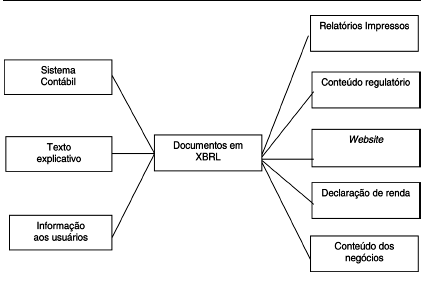
\includegraphics[width=.75\textwidth]{img/fluxo_info_xbrl.png}
\caption{Melhoria no fluxo de informação com XBRL. Adaptado de (\cite{hoffman2001xbrl}).}
\label{fig:fluxo_info_xbrl}
\end{figure}

Apesar de sua importância e crescente adoção, o \textit{XBRL Consortium} sentiu a necessidade de definir um modelo abstrato da XBRL (\cite{xbrl_preserve_promote_particite}) que facilitasse a compreensão da linguagem pelos profissionais da tecnologia da informação.Em 2012 foi proposto o \textit{XBRL Abstract Model 2.0}\footnote{\url{http://www.xbrl.org/Specification/abstractmodel-primary/PWD-2012-06-06/abstractmodel-primary-pwd-2012-06-06.html}} que consiste basicamente de uma versão estendida da \textit{Unified Modeling Language} (UML)\cite{booch2000uml} com objetivo de capturar os aspectos semânticos da XBRL.

No contexto da XBRL, uma ontologia é denominada como \textit{Taxonomia XBRL}{}. Consiste de um dicionário estruturado que resume o conjunto de conceitos contábeis/financeiros utilizado por determinada organização ou país. A partir de uma taxonomia é possível criar as \textit{Instâncias XBRL}, que contêm efetivamente os dados contábeis e financeiros que são assim trocados pelas empresas e as organizações envolvidas. Em síntese, a taxonomia é molde/validador para os documentos de instância XBRL.

A Figura \ref{fig:docs_xbrl} exibe como é estruturado um documento em XBRL. A \textit{Especificação XBRL} é responsável por definir as regras que governam a criação de arquivos
que seguem o padrão XBRL. Por outro lado, a Taxonomia XBRL é uma coleção de conceitos cobrindo uma área
de relatórios, sendo composta de um esquema, que compreende de um dicionário de termos escritos na linguagem XML Schema(\footnote{\url{http://www.w3.org/XML/Schema}}), e de linkbases, que são descrições de relacionamentos entre termos utilizando a linguagem XLink\footnote{\url{http://www.w3.org/TR/xlink/}}.

\begin{figure}[hbtp]
\centering
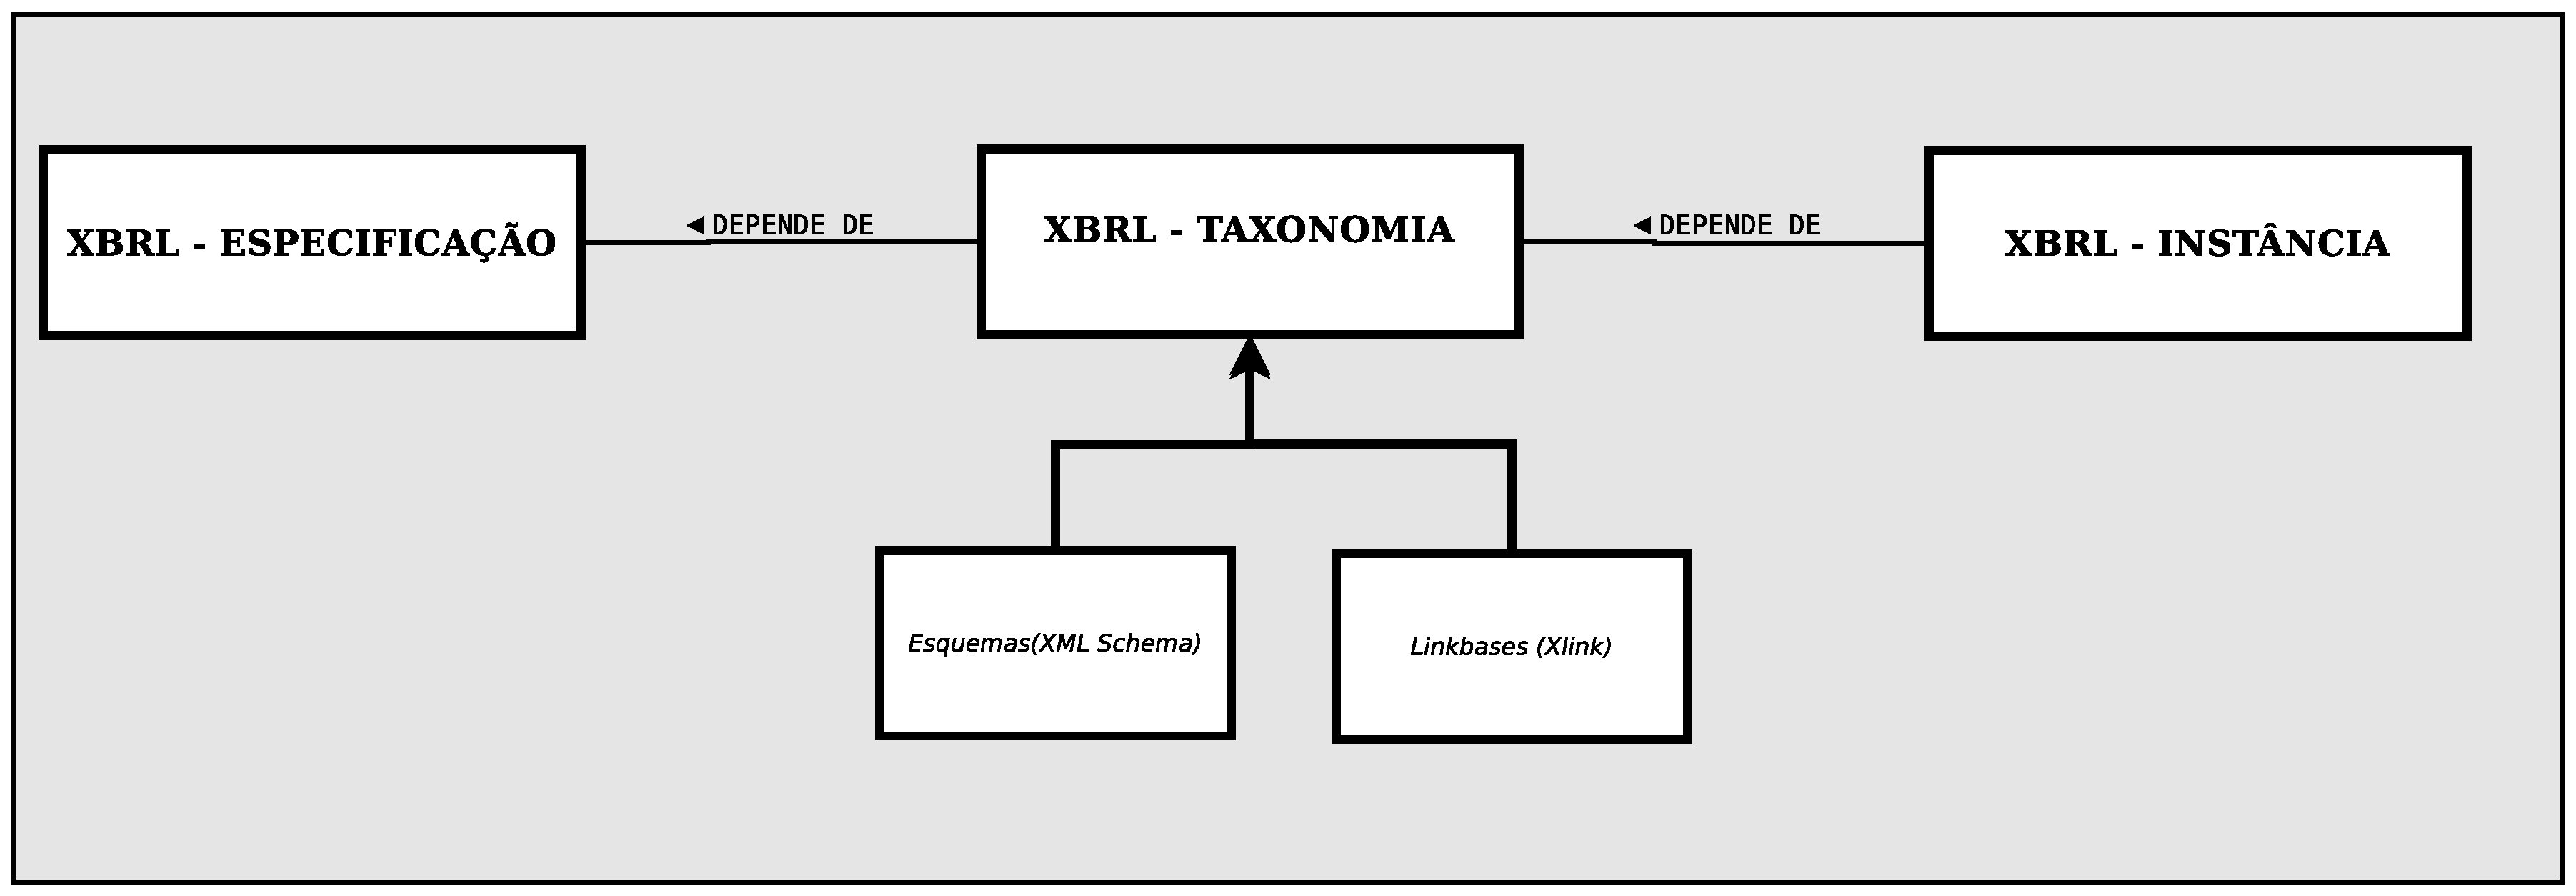
\includegraphics[width=1.0\textwidth]{img/documentos_in_xbrl.eps}
\caption{Documentos na estrutura XBRL.}
\label{fig:docs_xbrl}
\end{figure}

Conforme exposto, uma taxonomia em XBRL é representada através de um arquivo na linguagem XML Schema (\textit{.xsd}). A Figura \ref{fig:taxonomia_xbrl} demonstra como um determinado conceito é representado em uma taxonomia XBRL. Apesar de um arquivo \textit{.xsd} ser facilmente processado por computadores, o seu entendimento por parte dos seres humanos é mais difícil, sobretudo para profissionais que não tenham conhecimento prévio da XML. A Figura \ref{fig:arquivo_xsd} exibe uma parte de um arquivo \textit{.xsd} que corresponde à taxonomia proposta pela Secretaria de Tesouro Nacional\footnote{Disponível em \url{https://siconfi.tesouro.gov.br/siconfi/pages/public/taxonomia/taxonomia_list.jsf}}.

\begin{figure}[hbtp]
\centering
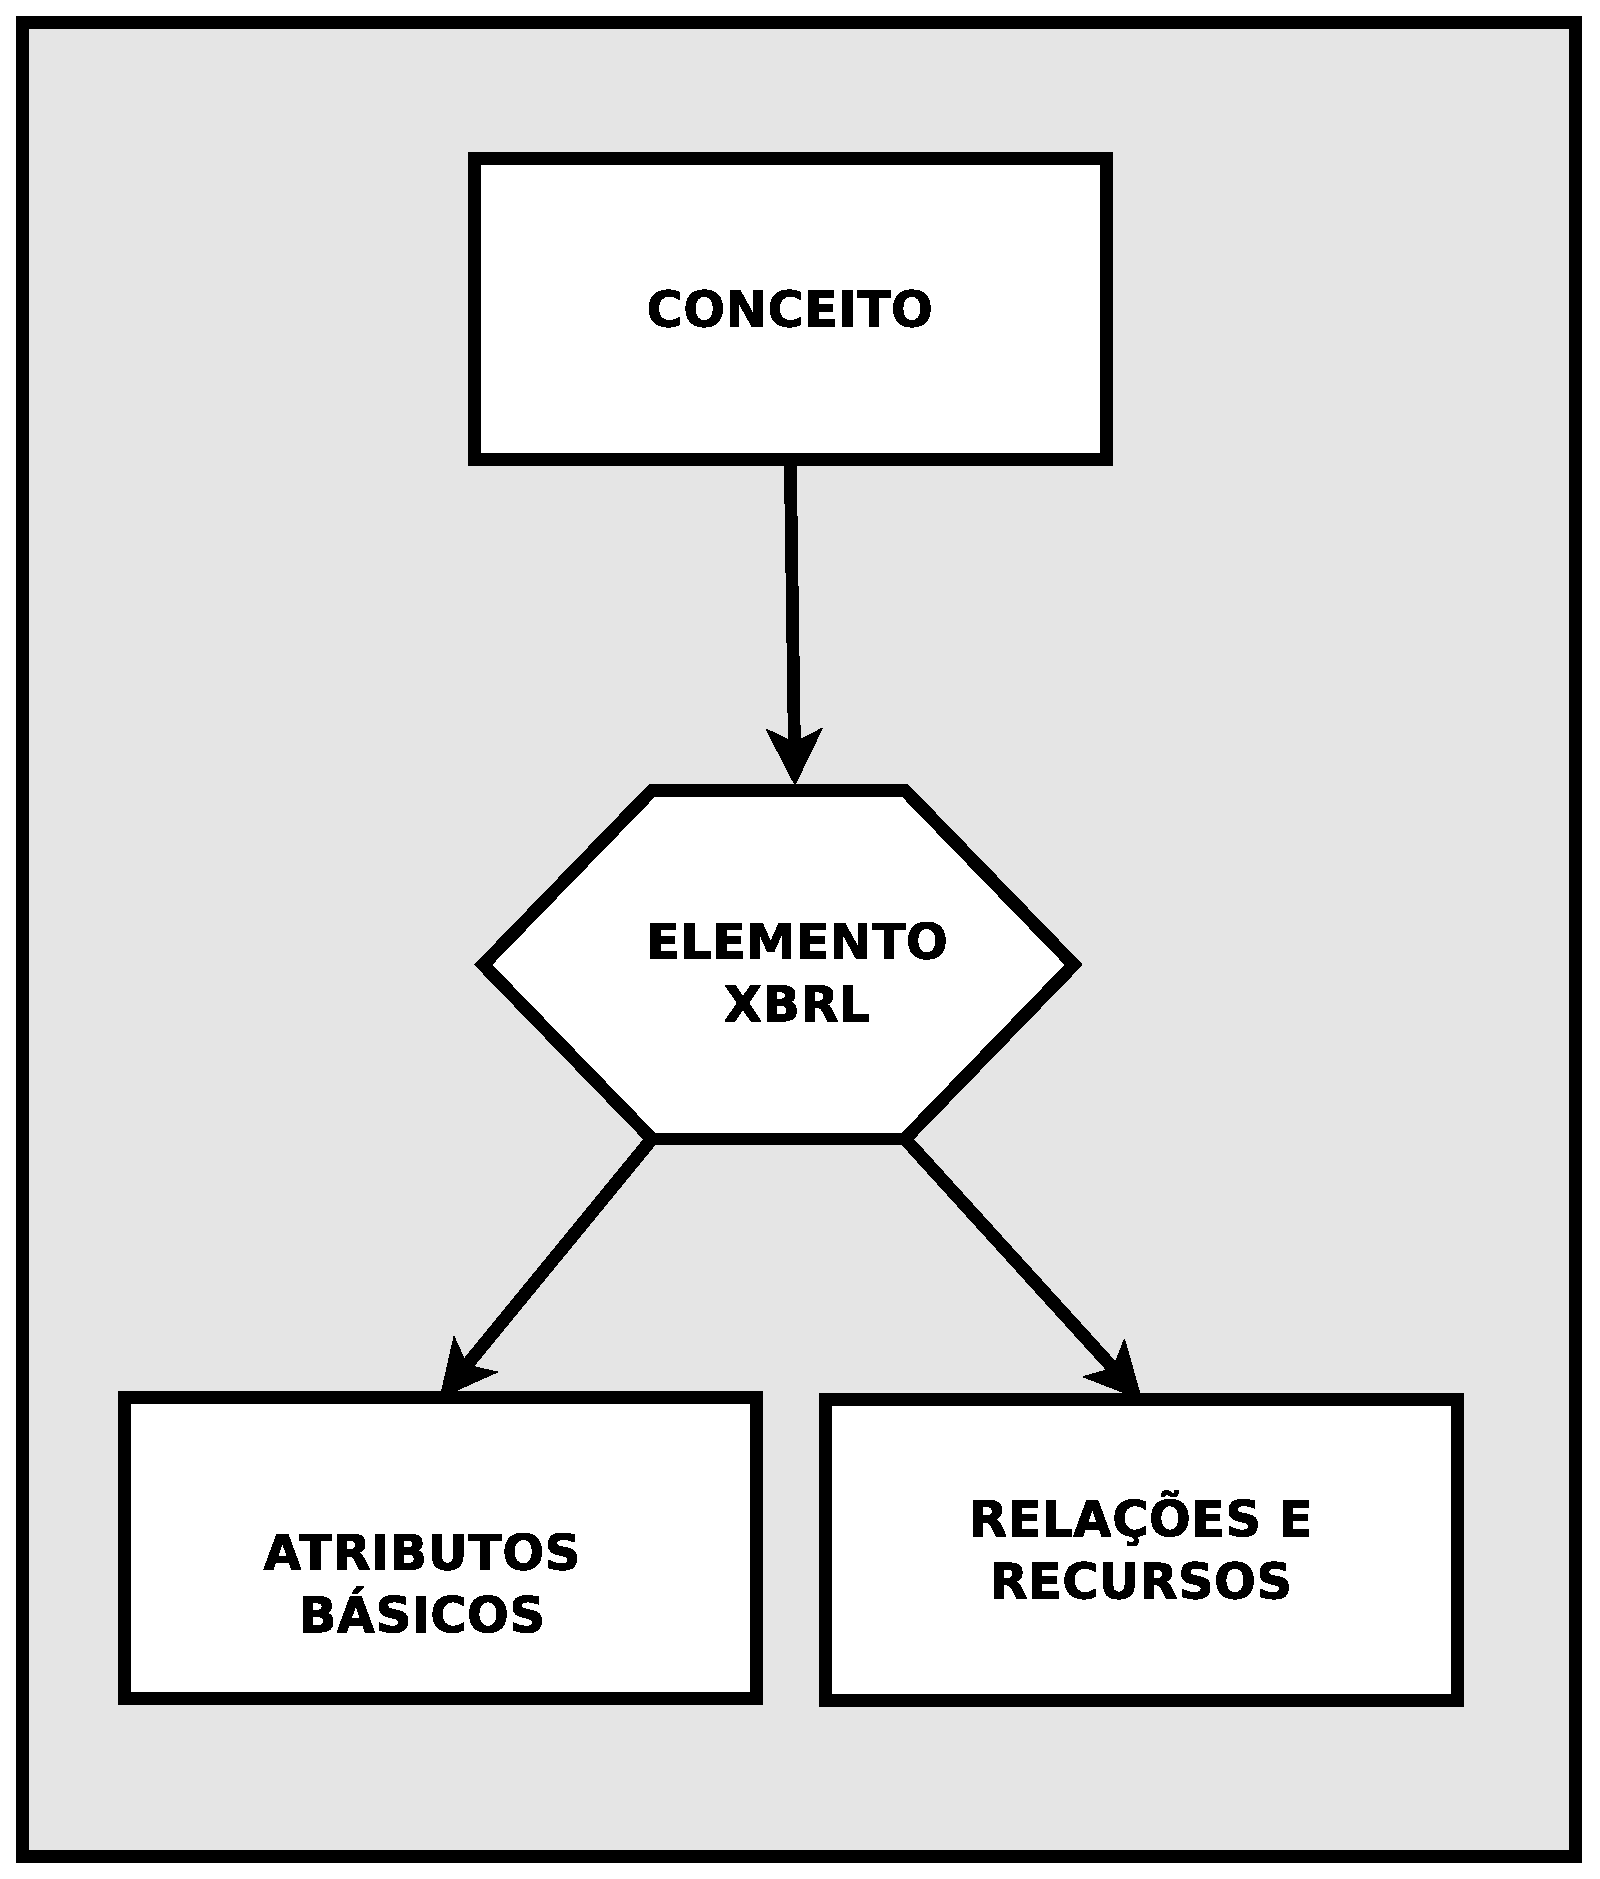
\includegraphics[width=.5\textwidth]{img/taxonomia.eps}
\caption{Modelo Conceitual da Taxonomia XBRL.}
\label{fig:taxonomia_xbrl}
\end{figure}

\begin{figure}[hbtp]
\centering
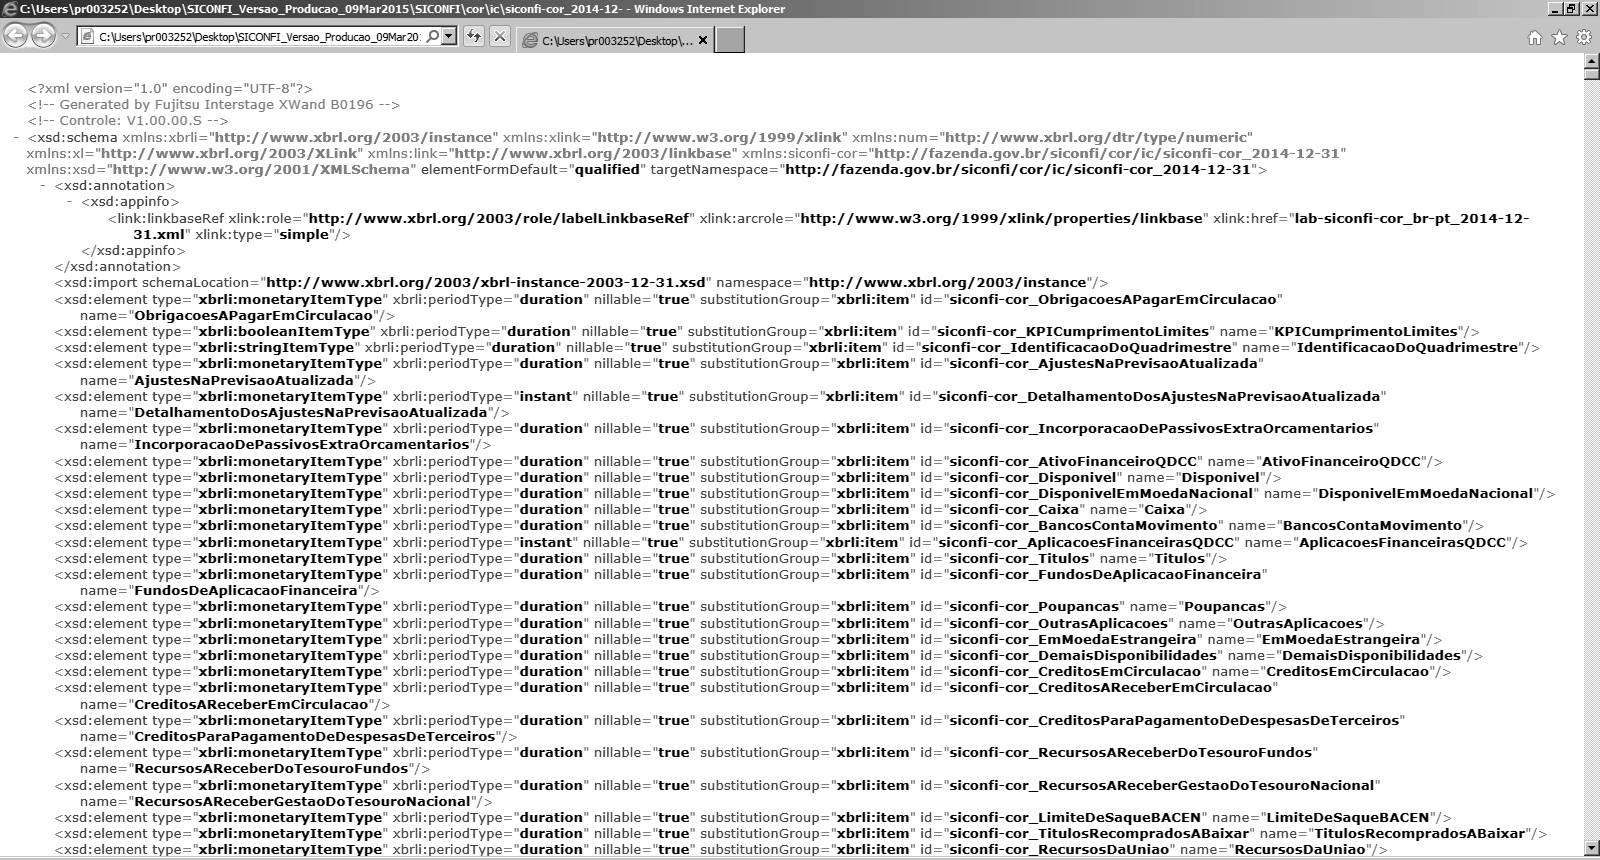
\includegraphics[width=.75\textwidth]{img/arquivo_xsd.png}
\caption{Taxonomia XBRL.}
\label{fig:arquivo_xsd}
\end{figure}

Suponha a comunicação entre uma equipe interdisciplinar utilizando apenas o arquivo exibido na Figura \ref{fig:arquivo_xsd}. Naturalmente haveria um prejuízo no processo comunicativo devido à inerente complexidade de um XML Schema. Desta forma, se faz necessário definir algum tipo de notação que facilite a comunicação entre os projetista de uma taxonomia XBRL, bem como propicie o desenvolvimento de modelos de taxonomia que poderia, através de ferramentas de \textit{forward engineering}, criar os arquivos \textit{.xsd}{}.

Um modelo abstrato deverá remover do seu escopo qualquer questão relativa à implementação do objeto modelado. Neste sentido, no caso de XBRL, o modelo abstrato deveria remover todas as referências a XML, o que não ocorreu no XBRL Abstract Model. Ademais, apesar da UML ser largamente utilizada entre os profissionais de Tecnologia da Informação, o seu uso para comunicação com os demais interessados muitas vezes não é o ideal (\cite{peixoto2008comparison}).

Neste contexto se faz necessário a proposição de linguagem conceitual para a XBRL com as seguintes características:
 \begin{itemize}
    \item Não contenha questões relativa ao XML
    \item Possibilite o desenho de aplicações que utilizem a XBRL
    \item Facilite a comunicação entre os diversos interessados envolvidos no domínio da XBRL.
 \end{itemize}

Nos próximos capítulos iremos revisar a literatura relativo à definição de ontologias, especialmente no domínio contábil e financeiro.

\chapter{Revisão da Literatura}
\label{ch:revisao}

No trabalho de \cite{Bosch:2013:APD:2575980.2575988} é apresentado um estudo sobre a criação de ontologias com base em XML Schemas. Arquivos no formato XML Schemas são utilizados por linguagem como XBRL para definir os conceitos a serem utilizados em determinado domínio. Neste sentido, todas as informações localizadas em um XML Schemas podem ser reutilizados a fim de reduzir a necessidade de criar ontologias de domínio a partir do zero. Os autores argumentam que o tempo e esforço economizados poderiam ser utilizados para acrescentar informação semântica inerente ao domínio, tendo em vista que este tipo de detalhamento não existem nos XML Schemas.

Em \cite{journals/ijcsa/Pierre08} há uma discussão sobre alguns dos problemas do uso de representações formais no domínio da contabilidade. O objetivo do autor era construir uma representação das informações financeiras de uma forma eficiente. Todavia, devido a própria maneira que a contabilidade é construída, basicamente de leis e normas, existem diversos problemas na representação dos elementos da mesma. Não obstante, Pierre considera a XBRL como uma boa alternativa para uma representação formal da contabilidade. O autor ressalta que a XBRL trouxe novos elementos para o processo de criação de relatórios financeiros: $(i)$ facilidade na produção e publicação das informações contábeis; $(ii)$ compartilhamento e possibilidade comparação partilha de informação; $(iii)$ verificação e certificação da informação; $(iv)$ ganho no processo de análise. Ele conclui que XBRL é bom padrão para armazenar informações, contudo, faz uma crítica ao padrão por não fornecer nenhuma formalização explícita de dados financeiros ou das normas contabilísticas.

Os pesquisadores \cite{lupacsc2010role} realizam uma análise do REA Framework\footnote{\url{http://reatechnology.com/}} como uma ontologia de contabilidade para sistemas de informação. Os elementos básicos do REA são recursos, eventos, agentes, fluxos, controle e \textit{duality} (\cite{mccarthy1982rea}). Os autores estendem o REA a fim de possibilitar a adição e compartilhamento do conhecimento.

Em \cite{gailly2007positioning} utilizou-se a UML para representar graficamente ontologias baseadas no REA. Os autores utilizaram metodologias tradicionais para a criação de ontologias para desenvolver o modelo proposto e argumentam que REA é uma ontologia de domínio do negócio. Eles concluem que linguagens conceituais tais como UML possuem a riqueza necessária para representar REA componentes ontológicos. Todavia, alguns detalhes dos elementos representados não são capazes de serem explicitados.

No trabalho de \cite{sugumaran2002ontologies} há a discussão da criação, uso e gestão de ontologias para modelagem conceitual. Eles também propõe um processo para gestão de ontologias. Os objetivos dos trabalho incluem demostrar a importância de ontologias na modelagem conceitual e propor um modelo baseada em heurística  para a criação de ontologias em determinado domínio. Eles observam que a maioria das ontologias são criadas manualmente e que não existe uma metodologia largamente aceita para construção das mesmas. O seu método de criação ontologia proposto é composto por quatro etapas. O primeiro passo é a identificação de termos básicos do domínio. Isto inclui duas eta-pau: a identificação dos termos mais frequentes e a identificação de sinônimos e termos relacionados. O segundo passo é a identificação dos relacionamentos. Existem três tipos de relações: relações entre termos básicos, relações entre ontologias, e as relações entre ontologias e sub-ontologias. O terceiro passo é a identificação de restrições e regras do domínio. O quarto passo é a identificação de restrições de nível superior. Estas restrições capturar o conhecimento de domínio. Os autores observam ainda que, enquanto a maioria das ontologias são construídos estaticamente, a maioria dos domínios, na verdade, evoluem com o tempo. O desenvolvimento de uma ontologia deve incluir esta evolução.

\chapter{Metodologia}
\label{ch:metodologia}

O processo de desenvolvimento deste trabalho pode ser dividido em quatro partes principais: $I$\textit{ - Revisão Sistemática da Literatura}; $II$\textit{ - Desenvolvimento da Linguagem}; $III$\textit{ - Construção da Ferramenta}; $IV$\textit{ - Avaliação}. Cada uma das etapas é detalhada nas próximas seções.

\section{Revisão Sistemática da Literatura}
\label{sec:revisao_sistematica}

Uma \textit{Revisão Sistemática da Literatura} - SLR (do inglês Systematic Literature Review) é uma
metodologia científica cujo objetivo é identificar, avaliar e interpretar
\textit{toda} pesquisa \textit{relevante} sobre uma questão de pesquisa, área
ou fenômeno de
interesse\cite{keele2007guidelines,wohlin2012experimentation}. Neste trabalho
será utilizada as diretrizes proposta \cite{keele2007guidelines} no qual uma
Revisão Sistemática deve seguir os seguintes passos:

\begin{enumerate}
  \item \textbf{Planejamento}
  \begin{enumerate}
    \item \textit{Identificar a necessidade da Revisão}
    \item \textit{Especificar questões de pesquisa}
    \item \textit{Desenvolver o Protocolo da Revisão}
  \end{enumerate}
  \item \textbf{Condução/Execução}
  \begin{enumerate}
    \item \textit{Seleção dos Estudos Primários}
    \item \textit{Análise da qualidade dos Estudos Primários}
     \item \textit{Extração dos Dados}
     \item \textit{Sintetização dos Dados}
   \end{enumerate}
  \item \textbf{Escrita/Publicação}
  \begin{enumerate}
    \item \textit{Redigir documento com os resultados da Revisão}
    \item \textit{Redigir documento com lições aprendidas}
  \end{enumerate}
\end{enumerate}


Dentro do escopo da dissertação, o desenvolvimento de uma Revisão Sistemática
tem por objetivo avaliar \textit{ferramentas para Relatórios de Negócio com suporte à linguagem XBRL}. \textit{Relatórios  de Negócio (Business Report)} é o produto final do  processo de divulgação pública de dados operacionais e financeiras de uma organização ou ainda a prestação regular de informações para os gestores dentro de uma empresa visado apoiá-los no processo de tomada de decisão.
\cite{lymer1999business}. Há uma terceira via da área de  Relatórios de Negócio está relacionada ao processo de prestação de contas por entes públicos aos governos nacionais.

Tendo em vista determinação da Secretaria do Tesouro Nacional, órgão
vinculado ao  Ministério da Fazenda do Brasil, que definiu o XBRL como
padrão para o envio de relatórios de prestação de contas pelos entes
federativos (estados e municípios) por meio do SICONFI – Sistema de Informações Contábeis e Fiscais do Setor Público Brasileiro \cite{nt_03_2013}, surge a necessidade por parte
daquelas organizações do \textit{desenvolvimento ou aquisição} de sistemas de
informação capazes de criar, processar e enviar informações no formato
XBRL. Um cenário onde tal situação ocorre tal necessidade é latente é em prefeituras de cidades de pequeno e médio porte que necessitam prestar contas via \textit{XBRL}, contudo
não possuem conhecimento ou tempo necessário para desenvolver alguma ferramenta que suporte a linguagem.

Neste sentido, verifica-se que existe a demanda por parte das organizações, especialmente as entidades públicas, de referências de qualidade sobre o assunto de \textit{XBRL}. Neste contexto, entende-se que uma Revisão Sistemática da Literatura - SLR  que avaliasse as ferramentas para Business Report que dão suporte ao XBRL pode \textit{subsidiar a tomada de decisão} por parte dos gestores públicos sobre a aquisição de tais ferramentas. Além disso, um trabalho neste sentido poderia subsidiar o desenvolvimento de novas ferramentas que venham preencher as eventuais lacunas existentes nos sistemas atuais. Ademais, traz o foco da comunidade científica sobre um assunto que vêm crescendo bastante nos últimos anos, dentre outros motivos, devido à necessidade das organizações públicas ou privadas de serem cada vez mais transparentes.

A presente \textit{SLR} reponderá as seguintes questões de pesquisa:

\begin{itemize}
  \item \textbf{$Q1$}: Quais são as ferramentas para Relatórios de Negócio que
    suportam a XBRL?
  \item \textbf{$Q2$}: Quais são os atributos comuns as ferramentas
    que possibilitem a comparação entre elas?
  \item \textbf{$Q3$}: Existem casos reais de utilização da ferramenta
    (Estudos de Casos, Whitepapers e etc)?
  \item \textbf{$Q4$}: Qual setor da economia (governos, medicina, setor financeiro) a ferramenta possui histórico de utilização?
\end{itemize}

\section{Pesquisa com Usuário}
\label{sec:survey}

Uma \textbf{Pesquisa com Usuário (Survey)} é um processo de
coleta de informações de ou sobre
\textit{pessoas} para descrever, comparar ou explicar seus
conhecimentos, atitudes e comportamento sobre um determinado
assunto\cite{fink2003survey}. Uma Pesquisa com Usuário geralmente é conduzida em retrospectiva, ou seja, tem como
objetivo avaliar a utilização por um determinado período de uma
ferramenta ou técnica \cite{kitchenham2009systematic}.

O objetivo desta etapa do trabalho é coletar informações e experiências de
pessoas que estão vinculadas com o processo de geração de Relatórios de
Negócio, especialmente àqueles que trabalhem com o envio de prestação de
contas. Esta faceta do Relatório de Negócio foi escolhida tendo em vista a
facilidade do autor em encontrar pessoas que trabalham neste processo.

Findada a Pesquisa com o Usuário serão coletadas informações e experiências que
podem subsidiar a definição das diretrizes para a construção de um sistema
para extração de relatórios de negócio.

\section{Prova de Conceito}
\label{sec:prova-conceito}

Com o objetivo de avaliar na prática o conjunto de diretrizes propostas, será
realizada uma Prova de Conceito mediante a construção de uma ferramenta para
extração de Relatórios de Negócio em XBRL utilizadas a diretrizes propostas
nesta dissertação. Tendo em vista o pouco tempo disponível para a construção da
ferramenta, esta apenas possibilitará a geração de um único relatório
denominado ``Matriz de Saldos Contábeis''. O processo de desenvolvimento da
ferramenta utilizada na Prova de Conceito será realizada no estilo agilista, onde seriam feitas algumas
iterações cobrindo os requisitos considerados mais prioritários.

\section{Avaliação}
\label{sec:avaliacao}

Com o objetivo de avaliar a diretrizes proposta por este trabalhado,
materializadas na ferramenta a ser construída como Prova de Conceito, será
realizada um Estudo de Caso. Segundo \cite{wohlin2012experimentation} um Estudo
de Caso é método empírico com o objetivo de investigar um objeto ou fenômeno em
seu contexto. A principal vantagem desta metologia é que os resultados são mais
realistas, todavia, estes resultados são difíceis de generalizar.

Neste sentido, propõe-se a utilização da ferramenta descrita na Seção \ref{sec:prova-conceito} como Prova de
Conceito para a geração do relatório ``Matriz de Saldos Contábeis'' no âmbito
da Empresa de Informática de Belo Horizonte - PRODABEL. A empresa foi escolhida
por conta do autor trabalhar na mesma e, portanto, possuir maior facilidade
para a condução do Estudo de Caso. Avalia-se ainda a aplicação do Estudo de
Caso em outros locais a fim de obter um maior conjunto de dados.

\chapter{Conclusão e Trabalhos Futuros}
\label{ch:conclusao_trab_futuros}

Conforme pôde ser observado, a XBRL vêm se tornando de fato um padrão para
intercâmbio de dados contáveis e financeiros. Contudo, apesar de sua crescente
adoção, exitem poucos trabalhos e ferramentas que suportem o processo de geração
de Relatórios de Negócio naquela linguagem.  Tentando preencher esta lacuna, o
trabalho ora proposto pretende definir um conjunto de diretrizes para criação
de ferramentas para a extração de Relatórios de Negócio que suportem a XBRL. Para tanto, a tabela \ref{tab:cronograma} descreve as atividades que serão realizadas para atingir este objetivo.

\begin{table}[!h]
\resizebox{\textwidth}{!}{%
\begin{tabular}{|c|l|c|c|}
\hline
\rowcolor[HTML]{C0C0C0}
{\textbf{\#}} & \multicolumn{1}{c|}{\cellcolor[HTML]{C0C0C0}{\textbf{Atividade}}} & {\textbf{Início(MM/AAAA)} } & {\textbf{Término(MM/AAAA)}}\\ \hline
1 & Revisão da literatura & 07/2015 & 08/2015 \\ \hline
2 & Ponto de Controle 01: reunião com o orientador & 08/2015 & 08/2015 \\ \hline
3 & Revisão da especificação XBRL & 09/2015 & 09/2015 \\ \hline
4 & Ponto de Controle 02: reunião com o orientador & 09/2015 & 09/2015 \\ \hline
5 & Revisão Sistemática da Literatura & 10/2015 & 12/2015 \\ \hline
6 & Ponto de Controle 03: reunião com o orientador & 10/2015 & 10/2015 \\ \hline
7 & Ponto de Controle 04: reunião com o orientador & 11/2015 & 11/2015 \\ \hline
8 & Ponto de Controle 05: reunião com o orientador & 12/2015 & 12/2015 \\ \hline
9 & Pesquisa com Usuário & 01/2016 & 02/2016 \\ \hline
10 & Ponto de Controle 06: reunião com o orientador & 01/2016 & 01/2016 \\ \hline
11 & Ponto de Controle 07: reunião com o orientador & 02/2016 & 02/2016 \\ \hline
12 & Ponto de Controle 08: reunião com o orientador & 03/2016 & 03/2016 \\ \hline
13 & Prova de Conceito: Construção da Ferramenta & 03/2016 & 04/2016 \\ \hline
14 & Ponto de Controle 09: reunião com o orientador & 04/2015 & 04/2015 \\ \hline
15 & Redigir a dissertação & 04/2015 & 05/2016 \\ \hline
16 & Ponto de Controle 10: reunião com o orientador & 05/2016 & 05/2016 \\ \hline
17 & Defesa da dissertação & 07/2016 & 07/2016 \\ \hline
\end{tabular}
}
\caption{Cronograma do projeto}
\label{tab:cronograma}
\end{table}


% Incluindo bibliografia:
\ppgccbibliography{./bib/bibliografia}
\end{document}
